%
% General structure for the revdetua class:
%

\documentclass[...]{revdetua}
\usepackage{graphicx}
%
% Valid options are:
%
%   longpaper --------- \part and \tableofcontents defined
%   shortpaper -------- \part and \tableofcontents not defined (default)
%
%   english ----------- main language is English (default)
%   portugues --------- main language is Portuguese
%
%   draft ------------- draft version
%   final ------------- final version (default)
%
%   times ------------- use times (postscript) fonts for text
%
%   mirror ------------ prints a mirror image of the paper (with dvips)
%
%   visiblelabels ----- \SL, \SN, \SP, \EL, \EN, etc. defined
%   invisiblelabels --- \SL, \SN, \SP, \EL, \EN, etc. not defined (default)
%
% Note: the final version should use the times fonts
% Note: the really final version should also use the mirror option
%




\begin{document}

\Header{1}{3}{Janeiro}{2021}{1}
% Note: the month must be in Portuguese

\title{Data Streams and Lossy Counting}
\author{Rodrigo Ferreira} % or \author{... \and ...}
\maketitle

\begin{resumo}% Note: in Portuguese
	Este artigo começa por contextualizar os conceitos essenciais para a compreensão dos problemas gerais relacionados com data streams, dos quais surge a necessidade de métodos eficientes de estimação de frequências.
Explica depois em detalhe um destes métodos, o \textit{Lossy Counting}, de Manku e Motwani. Começando pelo conceito, mostrando depois uma implementação da qual foram retirados alguns resultados e, por fim, uma discussão do impacto dos parâmetros.
\end{resumo}

\begin{abstract}% Note: in English
 This paper starts out by contextualizing the concepts essential to understanding the underlying problems that come from dealing with data streams, from which the need for efficient frequency estimation methods arises.
 Then it goes into detail on one of such algorithms, named \textit{Lossy Counting}, by Manku \& Motwani. First by explaining the concept, then showing an implementation from which we got some results and finally, a discussion on the impact of the parameters.
\end{abstract}
\section{Introduction}
\subsection{The Context}
With the current ever increasing use of technology, so too comes the ever increasing amount of data generated.\par
Much of this data takes the form of \textit{data streams}, huge amounts of pieces of data where although each piece might be very simple, the collection's size makes a complex whole.\par
There are endless examples of data fitting the model of \textit{data streaming}, but just to give a general idea, we will list a few:
\begin{itemize}
\item Sequences of queries on an Internet search engine;
\item Collection of transactions of a supermarket chain;
\item Data feeds from sensor networks;
\item Telecom call records;
\item Web server logs;
\item ...
\end{itemize}

The processing of this data model has 2 main differences from the processing of traditionally stored data.
\begin{itemize}
\item Across its lifetime a data stream tends to amount to more data than that seen in traditionally stored approaches.
\item Data streaming models require faster answers at any point in time.
\end{itemize} 

In many cases, data of the \textit{data streaming} model ends up indexed and archived in data warehouses regardless, like traditionally stored data, but, as it requires fast response times, it's impossible to "read" the entirety of the stored data every time an answer is required.  This creates the need to process items "on the fly", as they come, to obtain immediate information.\par
Due to this "on the fly" processing, output can be achieved at any point of the process if needed, there's no obligation to wait until the end of the stream.\par
It's also important that the processing method used is efficient, meaning it takes significantly less resources (space and time) to save the information needed, compared to the size of the input stream. This is all achieved only passing through the data stream once, most of the time.

\subsection{The Requirement}
A frequent requirement of such a model is finding the most frequent occurring data items, also known as the "heavy-hitters" problem.
The user imposes a percentage of the total number of data items and \textit{ideally} the algorithm will efficiently return only the items with a frequency that matches or exceeds the threshold declared.
\section{The Solution}
\subsection{Data streaming algorithms}
Over the years many algorithms were discovered (some even rediscovered), to deal with data of this format.\par
There are two main approaches to this problem.
\begin{itemize}
\item Counter based algorithms.
\item Sketch based algorithms.
\end{itemize}
Counter based algorithms are the simpler of the two, generally, counts are maintained for a varying subset of stream items.\par
Sketch based algorithms implement randomness, use multiple hash structures at times and do not explicitely store stream elements.\par
On this paper we will focus only on one counter based algorithm, the solution provided by Manku \& Motwani, commonly known as "lossy counting".


\subsection{Lossy Counting}
Lossy counting is one of the counter based algorithms, and as such, the way it works is more intuitive for most people, here's a brief explanation.\par
\begin{enumerate}
\item The user declares an $\epsilon$, or error threshold, from that, the size of a moving window $k$ is calculated like so: $k=\lceil\frac{1}{\epsilon}\rceil$.
\item The program is initialized with $N$ (total number of items seen) as 0, $Bucket\_id$ (id of each window of size $k$ read) as 1, and with $T$ (a data structure to keep track of a subset of items ($item\_name$, $est\_frequency$, $\Delta$)) empty.
\item It reads an item $i$, increments $N$ and checks if $i$ is in the $T$ structure, if so, increments its value in $T$ by 1. Otherwise inserts it with 1 as $est\_frequency$ and the $current\_bucket\_id - 1$ as $\Delta$.
\item Checks if the number of items read "filled" the window or bucket of size $k$, if so, for every item $l$ in $T$, if $l\_est\_frequency + l\_\Delta \leq current\_bucket\_id$, its entry is deleted. Once this is done, the $bucket\_id$ is incremented and the algorithm keeps on reading items.
\item If a user requests a threshold  frequency $s$, the program will return the entries $j$ in $T$ that satisfy $j\_est\_frequency \geq (s-\epsilon)N$.
\end{enumerate}
Steps 3-4 are repeated until there are no new items in the data stream, and only then does it pass to step 5 (assuming we're only allowing queries at the end).\\
Intestingly, for every entry of $T$, its estimated frequency (more like estimated counter) represents the exact frequency (exact counter) of the item ever since it was inserted to $T$ \cite{Manku},that's why items that enter the structure early get very accurate results. And the corresponding value of $\Delta$ is the maximum number of times that item could have occurred in the previous buckets/windows, that's why it remains unchanged after being inserted.\\
It's worth noting that for instance, in the previous explanation of the algorithm, frequencies entailed counter-like integers, but from this point forward, all mentions of frequency, whether exact or estimated, refer to the value from 0 to 1 or 0\% to 100\% achieved by dividing the "counter" by the number of items read, N (and also multiplying by 100 in the case of percentages).\\
Some properties can be derived from the nature of the algorithm \cite{Manku}, namely:
\begin{itemize}
\item It can find all items $x$ in a data stream that verify: $true\_frequency(x)>threshold$
\item The solution will contain no item $y$ such that: $true\_frequency(y)<threshold-\epsilon$
\item The estimated frequencies are less than the true frequencies by at most $\epsilon$.
\end{itemize}
Where an item x's true frequency at N items read is given by:
$$\frac{Exact\_Counter(x)}{N}$$
With $Exact\_Counter(x)$ being the exact number of times x occured up to N items read.\par
From these properties \cite{Manku} we can deduce that there will never be any false negatives (all items that verify the threshold frequency will be returned, as per property 1), but there might be false positives (elements whose frequency is between $treshold-\epsilon$ and $threshold$), elements returned that shouldn't be.\\
Interestingly, 2 versions of this algorithm are available, differing mainly by the fact that in one version, all items in the dictionary contain an individual $\Delta$ (the version explained), and in the other, all items share a common $\Delta$ given by $\Delta(i)=\lfloor{\frac{i}{k}}\rfloor$.
This other version was also presented by Manku, with the goal of avoiding the cost of storing individual $\Delta$ values.\par From now on, the original version with individual $\Delta$'s will be referred to as $ID$ while the shared $\Delta$ version will be referred to as $SD$.
Here's $SD$'s pseudocode \cite{Cormode}:

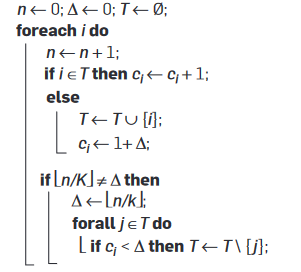
\includegraphics[scale=1]{pseudo.png}

\section{The Method}
In order to put the previously mentioned algorithms to the test, we had to implement them in Python and create some testing scenarios to get a better idea of their results.
\subsection{Code}
The code is divided in some python files.\par
First, there's $CharChain.py$, this file contains the class that represents the chain of characters which we will test on. Given a source string a length and a path, it will randomly generate a chain of characters and create a file in the text\_files folder, containing the chain itself on the first line (until a newline is inserted), and some valuable information in the following lines, such as the source string used, its size, exact counts, ordered ranks and a table to get a better overview of the exact frequencies.\par
Then there's $LossyCounting.py$ this file contains 2 classes $lossycounting\_sd$ and $lossycounting\_id$, representing the shared delta and individual delta versions of the lossy counting algorithm respectively. These classes get an epsilon and a path to the character chain file and apply the corresponding algorithm, it also gets the chain's exact stats present in the file to later output results for a desired threshold with detailed metrics like the relative and absolute error of the estimated and exact frequencies. It also compares the exact and estimated relative order of the items as well as the amount of false positives.\par
The file responsible for results is $Simulation.py$ here, there are 2 classes, $Simple\_Simulation$ and $Full\_Simulation$.
$Simple\_Simulation$ represents a simple test of one chain for both versions of the lossy counting algorithm, providing easy ways to assess and compare the results.\par
$Full\_Simulation$ is where the bulk of the work happens, it runs several tests of various sizes with different threshold and epsilon combinations, whilst acquiring important evaluation metrics. Despite the results being printed to files in the $test\_data$ folder, it also plots some stats at the end of its execution, which is where the graphics in this article came from.\par
These classes are the foundation of the code, apart from them there is also $AuxFunctions.py$ which contains some simple auxiliary functions, and $main.py$ which is where everything is run from.\par
The code is documented so this brief description will suffice.
\subsection{Testing circumstances}
The testing was done on several files of various sizes containing chains of characters separated by a space.
Six character chains were created for each input size from [100, 1000, 10000, 100000, 1000000, 10000000].
\begin{itemize}
\item A simple one generated with the source string "abcdefghijklmnopqrstuvwxyz".
\item One from the source string "aaaaabcdeeeeefghiiiiijklmnooooopqrstuuuuuvwxyz".
\item One where the first half was generated from the source string "abcdefghijklmnopqrstuvwxyz" and the second half from "aaaaabcdeeeeefghiiiiijklmnooooopqrstuuuuuvwxyz".
\item Another similar to the previous one but in reverse order.
\item One with the first half generated from "aaaaabcdeeeeefghiiiiijklmnooooopqrstuuuuuvwxyz" and the second half from "xyz".
\item And another similar to the last one but in reverse order.  
\end{itemize}

In the first one, every letter is equally likely to be picked at any point of the chain's generation, a truly fair random chain.
The second one favours vowels more than consonants.\par
The goal of the last four is to make a more realistic data stream, where frequencies can change drastically, this also allows us to see the impact of item order in the results of the lossy counting algorithm.\par 
Then, for every character chain, both versions of the algorithm were applied with different combinations of thresholds ([3\%, 5\%, 10\%, 15\%, 20\%]) and $\epsilon$ ([0.01\%, 0.1\%, 0.5\%, 1\%, 5\%, 10\%]) ignoring only tests where $\epsilon>threshold$. \par
The main thing evaluated was the $\epsilon$'s impact, so it was the subject of the outermost "for", meaning that every chain of every size and every threshold value was tested for each $\epsilon$ value, and then the results were printed to an individual file for each $\epsilon$ ($test\_data$ folder).\par
This was done because $\epsilon$ is the main parameter of the lossy counting algorithm and as such it makes sense to focus on its impact rather than something like the chain's size.\par
\section{Results}
The results obtained are all present in the $test\_data$ folder, and the following plots were obtained from running the program with the chains generated as previously discussed.\par
It's worth mentioning that these metrics were obtained by first averaging the stats of every item returned for each test case, and then averaging those average values for all tests of a given $\epsilon$.
The metrics are:
\begin{itemize}
\item Absolute error.
\item Relative error.
\item Total false positives.
\item Percentage of false positives.
\item Rank misplacement percentage.
\end{itemize}
Because this algorithm's objective is dealing with frequencies, the counts weren't used but were always translated to frequencies (both exact and estimated), so most calculations were done with percentages.\par
The absolute error being the absolute difference in percentage between the estimated and exact frequencies.\par
The relative error being the absolute error divided by the exact frequency, to get an idea of how big the error was compared to the correct value.\par
The total amount of false positives represents the number of false positives returned (items $x$ such that $s > true\_frequency(x) \geq s-\epsilon$), where $s$ is the chosen threshold.\par
The percentage of false positives simply divides the amount of false positives by the total amount of items returned.\par
And finally, the rank misplacement percentage represents the percentage of items returned whose estimated rank (relative order) is different from its exact rank.
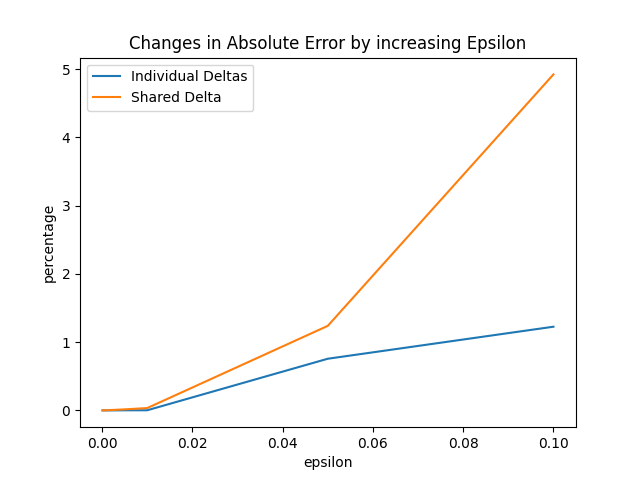
\includegraphics[scale=0.5]{absolute.png}
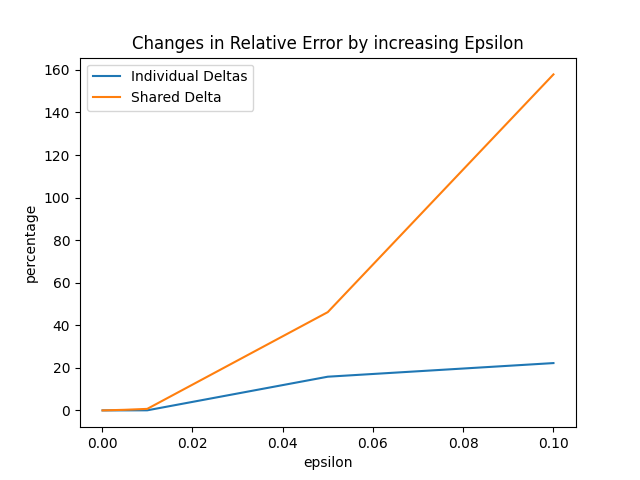
\includegraphics[scale=0.5]{relative.png}
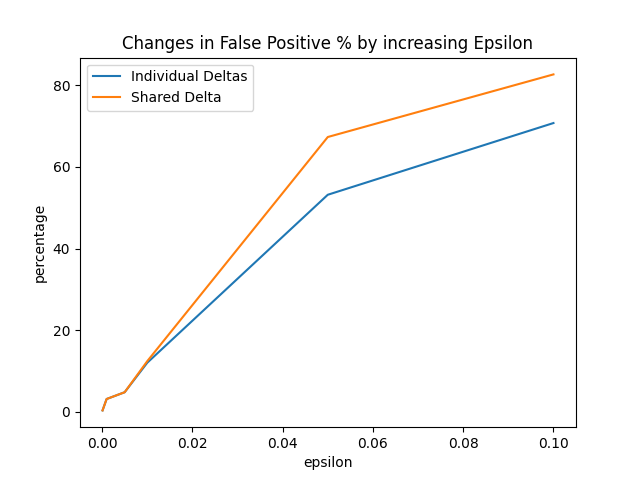
\includegraphics[scale=0.5]{false positive percent.png}
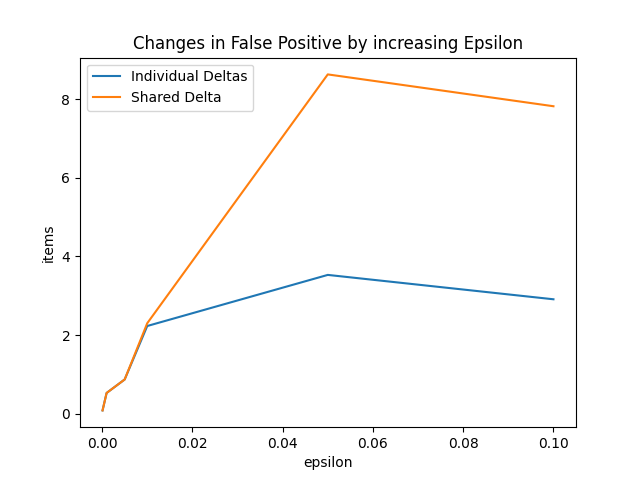
\includegraphics[scale=0.5]{false positive.png}
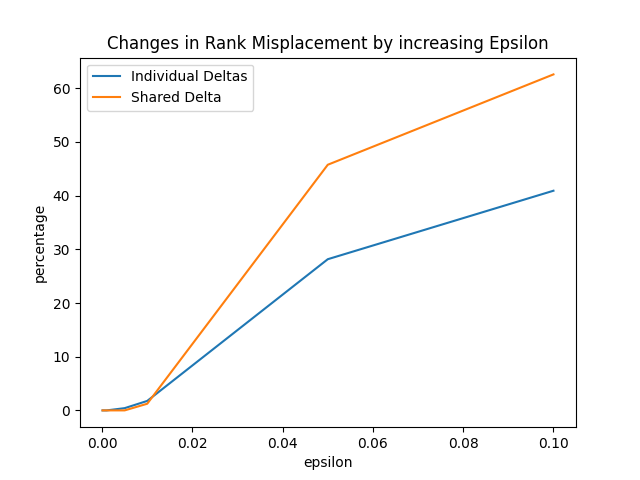
\includegraphics[scale=0.5]{rank misplacement.png}

\section{Observations}
We can make some observations from the results.
\subsection{Unexpected Results}
At first glance all graphics seem intuitive with results that should be expected, except for the case of the drop in the total number of false positives.
\par
This can be attributed to 2 factors.
First, the fact that for bigger $\epsilon$ values, more tests had to be ignored (following the threshold $s \geq \epsilon$ rule), this in turn gave more weight (less total results to average) to the remaining tests.\par
Second, given that the output can still be empty even for valid $\epsilon$ and threshold combinations (when there isn't any item whose frequency satisfies the threshold condition, no "heavy hitters" when it comes to the defined threshold), we end up giving even more weight to test cases where the heavy hitters had much higher frequencies than the other items, because there is a considerable difference in the items frequencies, it makes sense that the distribution is so "unfair" that even with a big $\epsilon$, none or few other items x could fit the false positive windows $s > true\_frequency(x) \geq s-\epsilon$, resulting in a smaller number of false positives.\par
These 2 factors severely reduce the amount of information retrieved from the tests, thus giving more weight to the results that remain, explaining the changes in the plot.
\subsection{Amount of items returned}
First it's easily noticeable that the $ID$ version of the algorithm returns considerably less items than its $SD$ counterpart, to be more precise, $SD$ returns more false positives.
This can be seen in the files generated from the tests, but also in the plots. \par
While both have an increase in false positive percentage, we can see that in raw number of items, $ID$ returns significantly less false positives than $SD$ as $\epsilon$ increases.
\subsection{Errors}
As expected, the errors grow as we allow a bigger margin for error, resulting in smaller buckets.\par
The $ID$ version outperforms the $SD$ version when it comes to errors.
The inability to pinpoint in which bucket an item  entered the structure due to the lack of individual delta values causes the guesses to be more inaccurate, and as such, the $SD$ version tends to overestimate frequencies more than its $ID$ counterpart.

\subsection{The Chains}
From the data in $test\_data$ we can see that the chain's size wasn't that impactful regarding the errors.\par
It was expected that when building each chain as a result of the concatenation of various chains with different source strings, the algorithm wouldn't be as accurate. Because using only one chain, when there are characters that are very likely to have a high frequency (due to their duplicates on the source string and consequently higher probability) they are very likely to show up in one of the initial buckets, and due to their high frequency, once they enter the structure keeping track of the counts, it's very unlikely that they will leave, thus making its estimate more precise.\par 
Thus, when using this mixed chain approach it's very likely that that character will have significantly different frequencies for each chain, making the data stream more "unpredictable" or "chaotic". \\This, in turn, makes it possible for the character in question to leave the structure keeping track of the counts, which as we know, will cause imprecision later.\par
This wasn't very present in most of our tests because most of the $\epsilon$'s used resulted in a decently sized window, with the smallest being of size 10 (for $\epsilon=10\%$). For the instance of the alphabet, which only has 26 different items, the number of deletions wasn't very big (comparatively) and thus the errors were around those calculated for instances using  a simple source string for most cases.\par
Additionally, we were asked in this assignment to find if in a random chain with uniform distribution any letter had a frequency higher than 5\% or 10\%?\\
To solve this we simply run the lossy counting algorithms on a chain generated from "abcdefghijklmnopqrstuvwxyz" with a small $\epsilon$ value like 0.1\% (0.001 as a float) and the desired 5\% (0.05 float) or 10\% (0.1 float) threshold.\\
To briefly answer this, in smaller test cases, some letters did have a frequency higher than 5\%, but as the input size grew, their frequency converged to $\frac{1}{26}$ as expected.\\
The chains built from the other source strings generated far more interesting and relevant distributions (in the sense of the "heavy hitters" problem). 

\subsection{Parameters}
Regarding the parameters themselves, the threshold is obviously chain dependent, depending on the frequencies of the data stream in question, there may or may not be items that fulfill the threshold requirement.\par
The parameter $\epsilon$ however, was generally seen as the most important overall.\par
A lower $\epsilon$ leads to much smaller errors, as expected, since $bucket\_size=\lceil \frac{1}{\epsilon} \rceil$, when $\epsilon$ is smaller, the bucket size will be bigger, meaning less possible deletions from the main data structure, which is what causes inaccuracy most of the time.\par
Likewise, higher $\epsilon$ will lead to bigger errors, as the bucket size is smaller, there will be more deletions, however there is a silver lining, the structure will have less items at any time as more deletions occur, so it will take up less space (not very meaningful in this case where the size of the max set of possible items is 26, the letters of the alphabet).
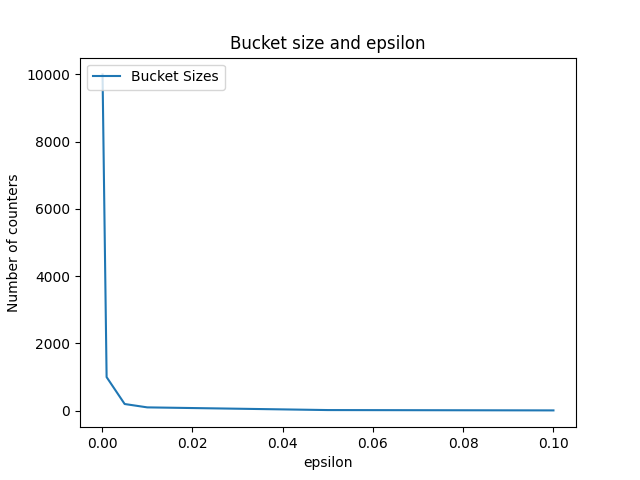
\includegraphics[scale=0.5]{bucket size.png}



\subsection{Versions}
When it comes to the algorithm versions, the results were clear, the individual delta version came out equal or ahead in pretty much every test and metric, as expected, though this came with the cost of additional memory for tracking every $\Delta$ value, but as mentioned regarding $\epsilon$, the maximum amount of different items possible in this case was 26, so the memory "wasted" was negligible. In a real world scenario though, with many different item types, it might be worth to trade off some accuracy for memory space.\par
The biggest problem of the $SD$ version is the amount of false positives, it may perform slightly worse in other metrics too but this one is where we can really tell which version is more accurate.

\section{Conclusions}
We conclude that the area of algorithms regarding data streams is very important in today's age as new (and even old) approaches surface constantly, each with their positive and negative aspects and significantly different algorithms. As we saw, both versions of the lossy count produce satisfactory results passing the data stream once, but with some trade offs regarding memory and accuracy.

\bibliography{bibliografia}
\end{document}
